\section{Common Network Resource Exposure} \label{sect:cnre}

This paper seeks to explore aggregate network resource catchments --- the set of
users exposed to the same set of web resources as each other across a given set
of domains. We introduce a new similarity measure, which we have coined common
network resource exposure (CNRE), to quantify the extent to which two clients
are exposed to the same network resources. Inspired by the Jaccard index CITE,
CNRE between two clients, $C_1$ and $C_2$, is defined as follows:

\[ \textrm{CNRE}(C_1, C_2) = \frac{ \sum_{i}^D  m_{i} (r_{1_i}^{-1}+r_{2_i}^{-1})}{ \sum_{i}^D (r_{1_i}^{-1}+r_{2_i}^{-1})} \]

where $D$ represents the intersection of measured domains between both clients, 
and $m_{i}$ is 1 if $C_{1}$ and $C_{2}$'s
$i$\textsuperscript{th} domain answers match (otherwise zero). The values
$r_{1_i}$ and $r_{2_i}$ represent the fraction of all measurements (across the
entire dataset) that matched $C_1$'s and $C_2$'s DNS answer for that domain,
respectively. For example, if $C_1$'s answer for domain $i$ appeared 900 times
across the 9024 times it was tested in our dataset (once by client), 
\RF{This is a bit confusing, we said we have 10,274 clients with Atlas}
\(r_{1_i} =  900 / 9024\), or 0.09973 (\emph{i.e.} roughly 10\% of the answers). 
In other words, $r_{n_i}$ captures the
\emph{rarity} of the DNS answer received by client $C_n$ for domain $i$.

In our calculation of CNRE, we use the inverse of $r_{n_i}$ to add increased
weight to the impact of a mismatch on rare answers. CNRE is therefore designed
to be higher between clients with more matching rare answers. As it is
ultimately a measure of similarity between clients, CNRE values range from 0
through 1, with 1 being the most similar. To ease discussion in the remainder of
this paper, here we also define \emph{distance} as \(1 - \)CNRE unless otherwise
noted.

\begin{figure}
    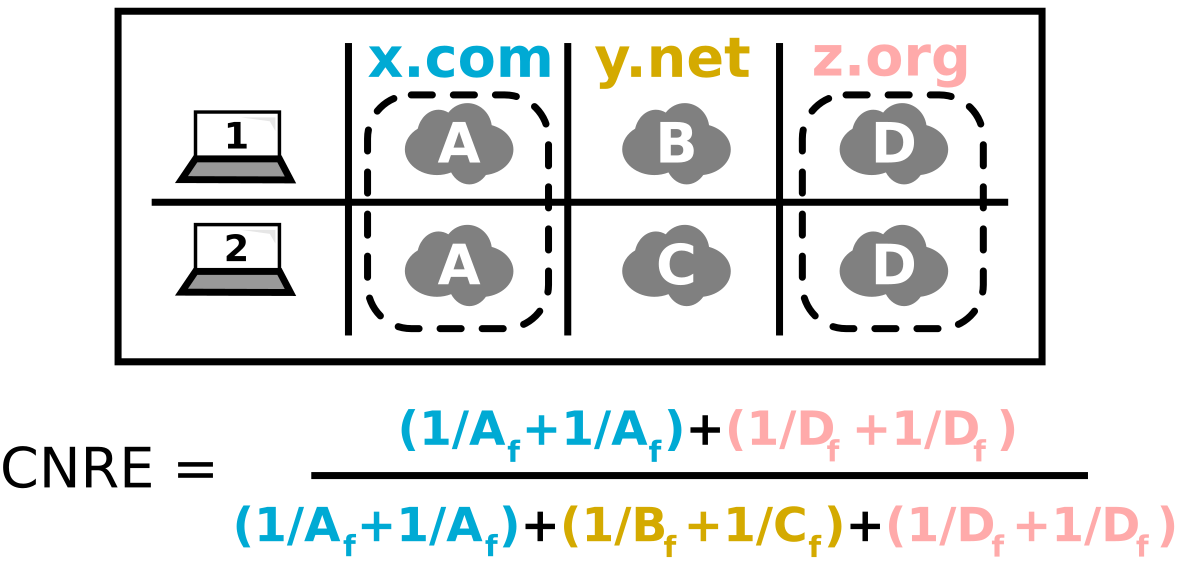
\epsfig{file=figs/cnre.png, width=1\linewidth}
    \caption{diagram illustrating CRNE}
    \label{fig:cnre}
\end{figure}

An example of CNRE calculation is shown in Figure \ref{fig:cnre}.
\RF{TODO: diagram explanation or remove the diagram?}

\begin{figure}
    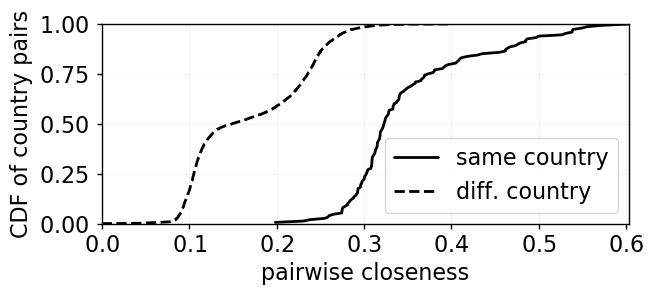
\epsfig{file=figs/country_cdf.png, width=1\linewidth}
    \caption{“High” closeness (90th percentile?) vs \# domains measured}
    \label{fig:90cnre}
\end{figure}

TODO: get 90th percentile plot and write about it

\begin{figure}
    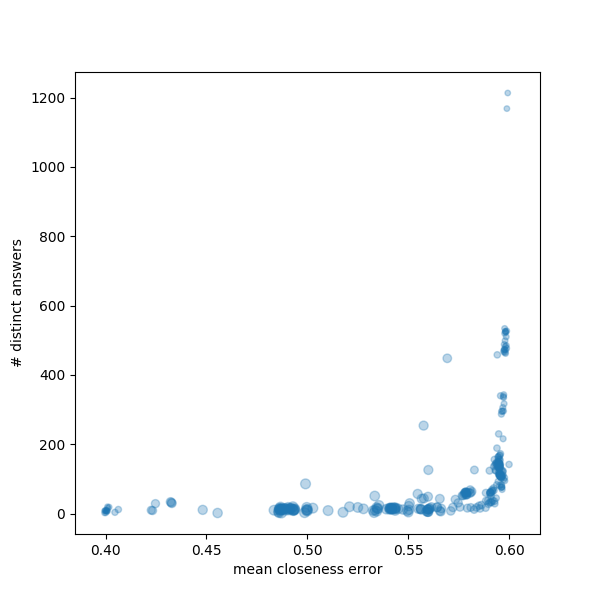
\epsfig{file=figs/domain_error.png, width=1\linewidth}
    \caption{Mean domain error vs \# of distinct answers observed from domain
    (one point per domain).}
    \label{fig:domerr}
\end{figure}

We pause here to address potential bias given toward individual domains. As CNRE
calculation gives increased weight to rare answers, there is the possibility
that the allocation patterns of large providers (who often have more answer
variety related to the scale of their networks) may dominate the results. This
would be detrimental to the main purpose of CNRE --- a supposedly aggregate
measure --- as it would ultimately revert to essentially measuring a single
provider, which is a well explored topic. To determine whether this is occurring,
we calculate the \emph{domain error}, for a single domain, as follows: Given a
pair of clients, first, find their CNRE normally. Next, let us set $d$ to be 1
if the DNS answer for the domain of interest matches between the pair of
clients, and otherwise 0. Finally, the domain error is the absolute value of \(d
- \)CNRE. In Figure \ref{fig:domerr}, we plot this, with each
point representing the mean domain error for a given domain across
the entire set of client combinations. 

With domain error, we simply capture how different the CNRE would have
been had that domain been the only one used in CNRE's calculation. A \emph{low}
mean domain
error --- close to zero --- implies that the domain is dominating over the
CNRE. A \emph{high} mean domain error --- close to one --- implies that the domain has little impact
on CNRE's value. A mean domain error close to the middle --- 0.5 --- is ideal,
as it implies that the domain is neither dominant nor irrelevant. We see in
Figure \ref{fig:domerr} that domains with many answers (and hence increased rarity per
answer) actually have the highest error. Further, the range of domain error
across all domains spans roughly from 0.4 to 0.6, indicative of the absence of
substantial bias towards any given domain in our approach.
